% Chapter 2

\chapter{Background Research} % Chapter title

\label{ch:background} % For referencing the chapter elsewhere, use \autoref{ch:background}

%TC:ignore
%This is the Background chapter, it should be approximately 4,000 Words in total.
%SRAM-PUF section should be approximately 1,500 words longs
%Fuzzy Extractor section should be approximately 1,500 words long.
%Forward error correction subsection should make up approximately 500 words.
%Cryptographic Hashing subsection should be about 500 words long.
%Networking section should be 1000 words in length.
%TC:endignore
%-------------------------------------------------------------------------------

The intention of this project is to investigate and implement in full - or in
part - a prototypical networked device that can be authenticated using a \gls{puf}.
As explained in the introduction, there are three areas under investigation.
In this chahpter are the findings from preliminary research undertaken for each
of the three areas. This is the foundation which supported the eventual system
design that will be discussed in the next chapter.

\section{Identity and Authentication}

Verificaton of identity is fundamental to this project, and so related concepts
and foundations should be explored. Firstly, it should be noted that
authentication is a different concept to authorization and accounting, although
the three together (AAA-security) are often considered as a whole, the focus in
this project is Authentication only.

\subsection{Challenge-Response}

In this project, \gls{cra} is foundation for authentication of device identity.
\Glspl{cra} isa commonly used concept in the authentication of devices on a
network. The concept is that the device to be authorized (hereby known as the
\emph{Supplicant}) is challenged by the device that controls access to the
network (hereby known as the \emph{Authenticator}). For each device to be identified
correctly, there must be at least one \gls{crp} associated with
each device and the supplicant must respond
with its correct response, otherwise access to the network is denied.

In the simplest case this could be as simple as a basic password check with a
unique password associated to each device/user. Thus, mutual authentication by a
shared secret is obtained.
However, if an attacker
can eavesdrop the communications channel, they can also see the password sent and
use a replay attack to gain access by spoofing the response of the original
supplicant. To make the system more secure, many \glspl{crp} can
be generated, thereby requiring an attacker to record all possible pairs to be
guaranteed access to the system. The probability of one-time access is
inversely proportional to the number of pairs, such that with sufficient pairs
the reply attack can be made statistically impossible.

There is one important complication; if a response can be
partially guessed solely through analysis of patterns in the ciphertext a
challenge generates (called information deduction) this weakens the system.
Therefore correlation of the challenge to the response should
be as near to the Shannon entropy limit as possible.

\subsection{Authentication Factors and Inherited Identity}

In network communications within a shared medium, the identities of the communicating devices
must be explicitly made so that they can be read by the intended recipient.
However, without security procedures in place, it is very simple and entirely
possible for any device
to claim the identity of another since there is no way to verify its provenance.
Thus, in mature networks some form of authentication protocol is introduced.
Authentication is generally performed using authentication factors, these can be stated
succinctly as one of three types;

\begin{itemize}
\item Knowledge - what you \emph{know}.
\item Ownership - what you \emph{have}.
\item Inheritance - what you \emph{are}.
\end{itemize}

In most cases of network authentication the first two factors are used, sometimes in combination.
In the case of knowledge factors examples include passwords and \glspl{pin}. In the case of
ownership factors, examples include \gls{rfid} tags and smart-cards.
These are extensively used for
current \gls{lan} authentication systems, for example the old \gls{wep} security scheme for the
IEEE 802.11 standard (branded as `Wi-Fi') required a password 10 to 26 Hexadecimal digits to
be physically entered by hand. In fact, secret keys of this type form an
integral part of hardware cryptographic primitives in conventional methods of authentication.
These necessarily rely on the digital storage of secret keys in non-volatile memory,
which has proven vulnerable to reverse engineering and side channel attacks.

Although less common, due to its more physical nature, Ownership factors include the `VideoGuard'
viewing cards that must be inserted into a set-top-box in order to authenticate the device over
a \gls{ppp} connection through the \gls{pots} to access encrypted digital
satellite or cable television channels. Ultimately these systems also rely on
the digital storage of keys, however, they are stored
within the smart-card and not the device itself. If an exploit is found, new protocols with changed
smart-card designs can be implemented and replacements distributed to upgrade the security of the system.
This incurs a significant additional expense, but allows for far greater longer-term security.

In contrast, inheritance factors are very uncommon in authentication of network devices, and
more usually are used to authenticate users themselves in the form of biometrics such as fingerprints,
iris-scans and facial recognition.
The advantages of inheritance factors over traditional methods for networked devices should
be clear;
\begin{itemize}
\item Increased Convenience - Automates process, nothing to be forgotten or misplaced by the users
\item Increased Security - No passwords on scraps of paper, or smart-cards in wallets to be stolen,
  and nothing is easily guessable or easily duplicated.
\item Increased Accountability - Auditing and post-factum reporting are stronger, as identities are harder to forge or alter.
\end{itemize}

While humans and other biological systems have biometrics that can be used in this way, it is
less obvious that electronic hardware systems can make use of Inheritance factors.
\Glspl{puf} are an enabling technology that can allow this.
By making use of them we can transfer much of
the beneficial techniques found in the application of
biometrics to user-centric security systems to
the topic of of device-centric authentication.

\section{PUFs \& SRAM}

The first thing required for a \gls{puf} based authentication system is a \gls{puf}.
Introduced in 2002\cite{pappu2002puf},
\glspl{puf} can be built from a wide variety of technologies.
Some have
electronic construction, some not, and new designs seem to appear every year.
Of those \glspl{puf} that are created from electronic circuits, there are some
that can use off-the-shelf components and some that must be custom made in
silicon. There are some that are delay based\cite{maiti2010large} and some that
are based on memory state meta-stability.
\gls{sram} \glspl{puf} that use the meta-stability of the standard six transistor
\gls{sram} cell (see \autoref{fig:sram}) were initially proposed by
Guadardo\cite{guajardo2009puf}, and are the focus of this project.

\begin{figure}
  \centering
  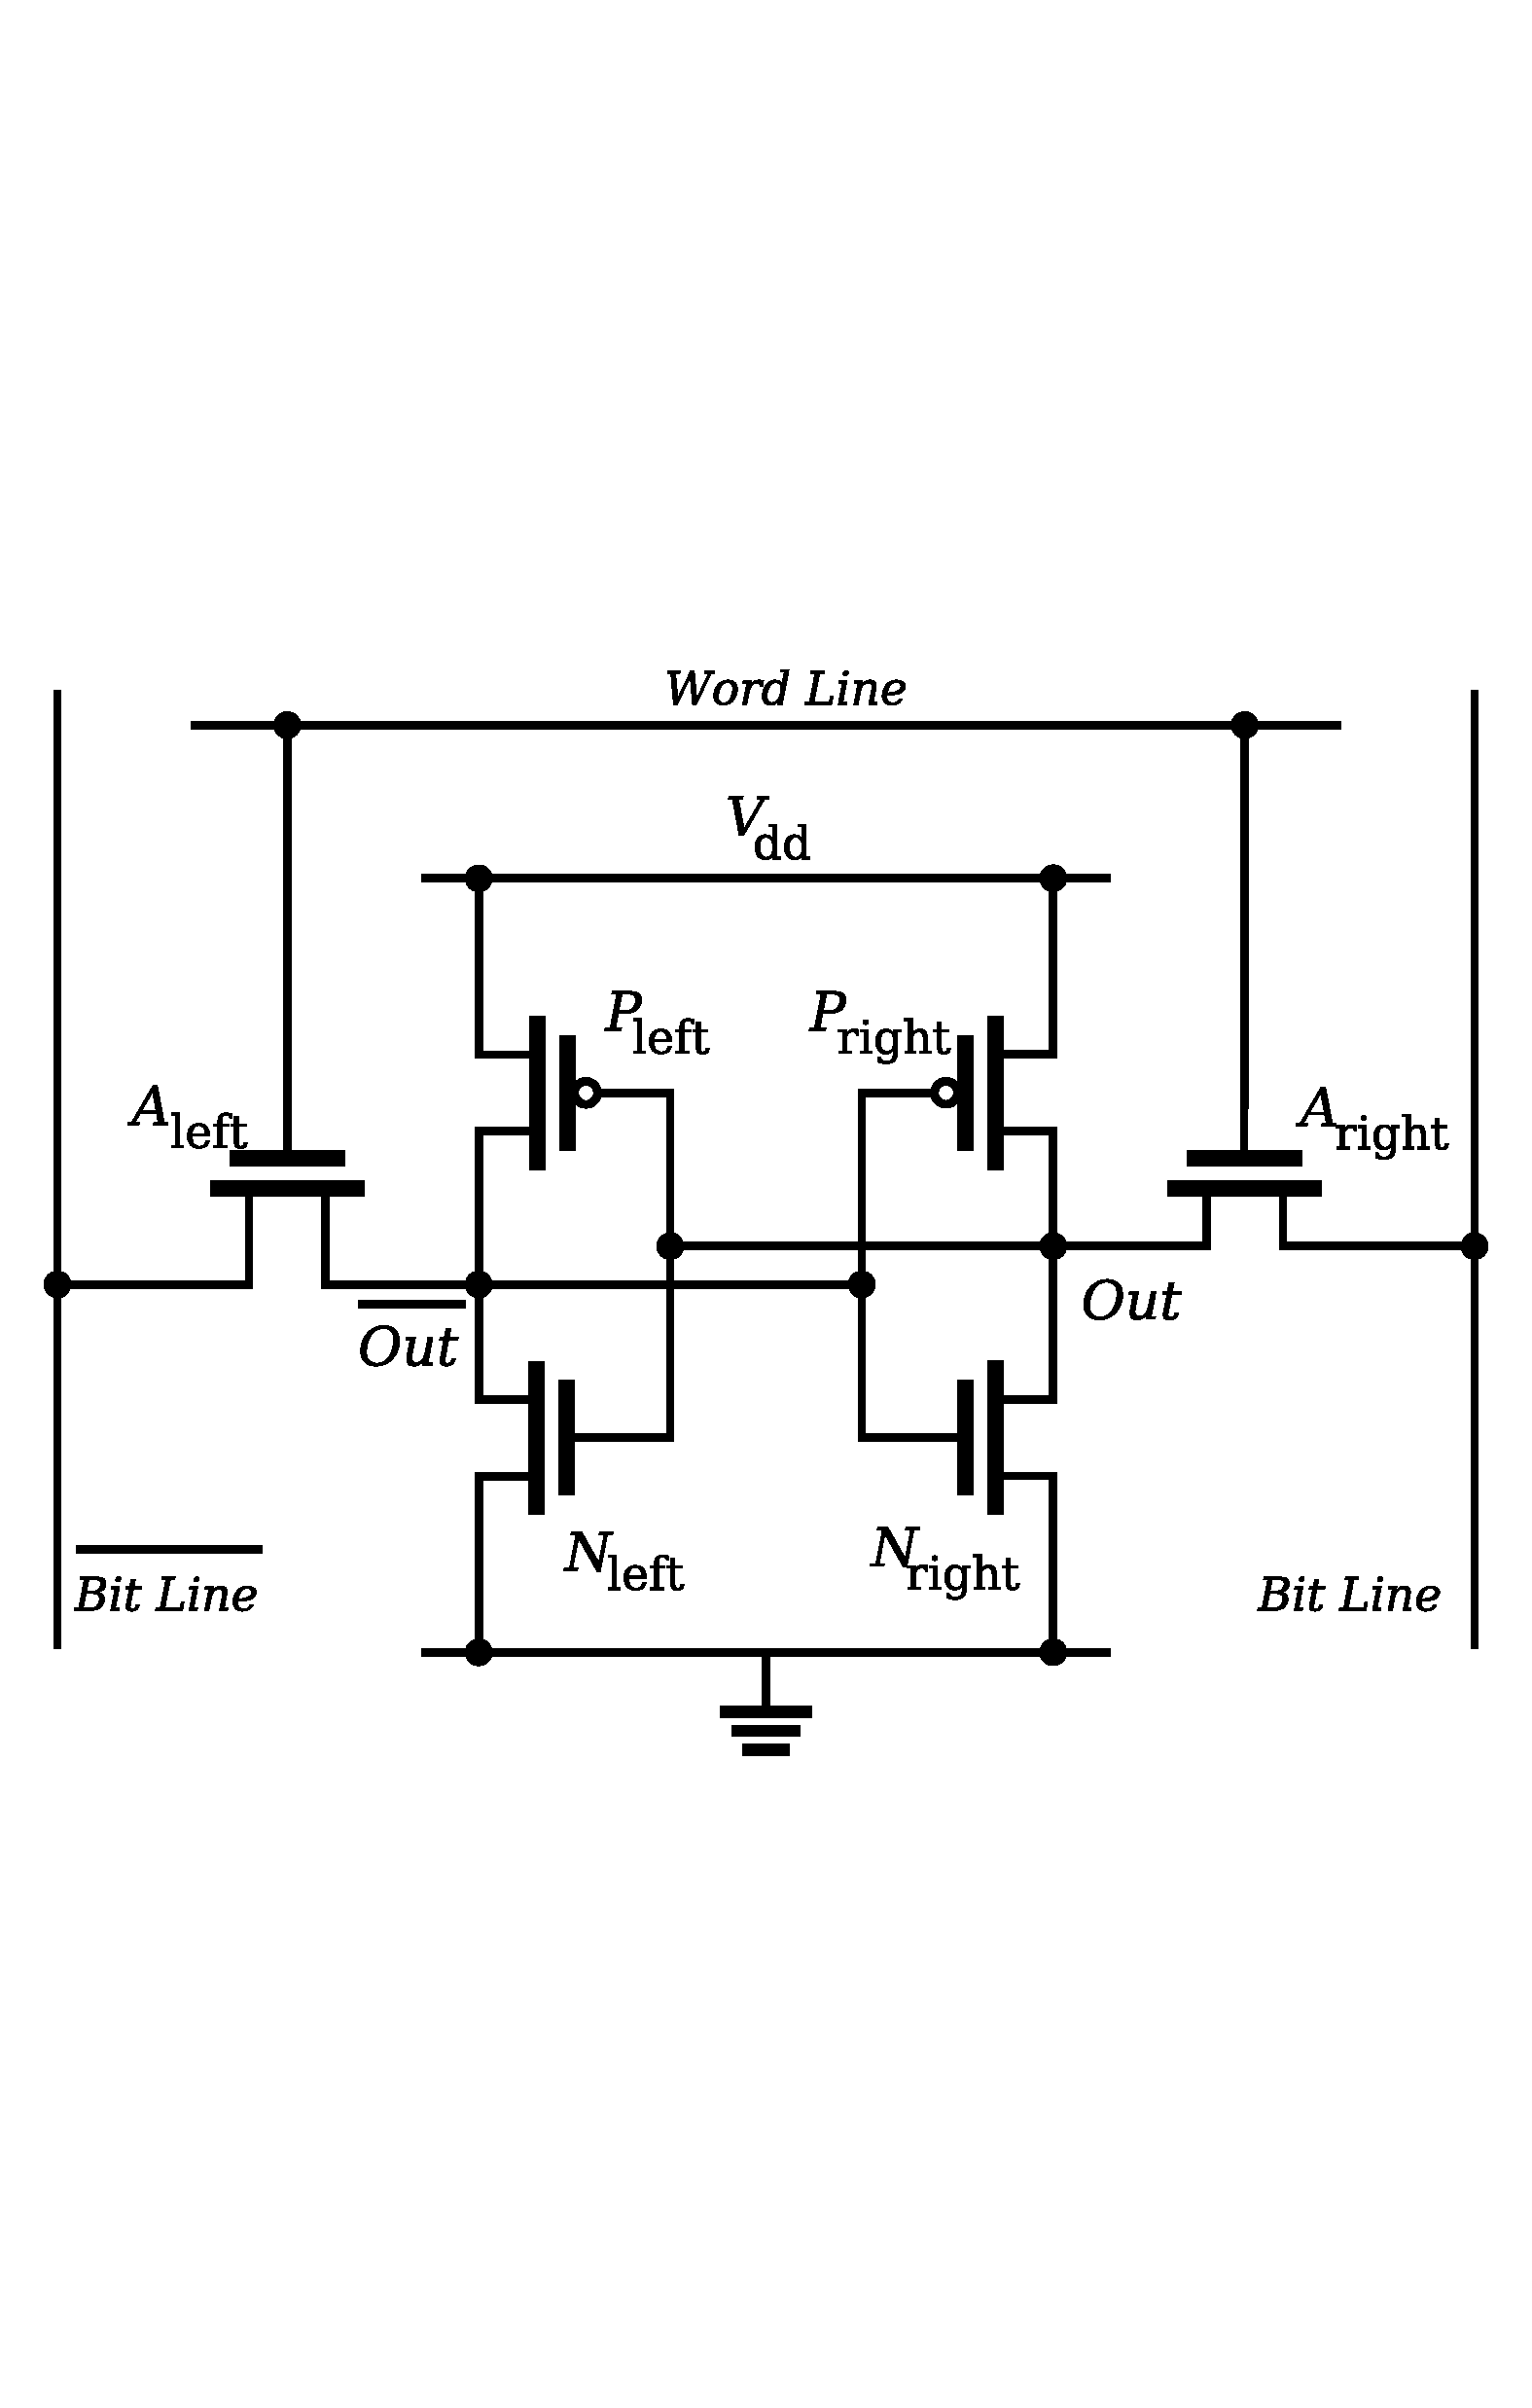
\includegraphics[scale=0.4, trim=0 300 0 300, clip]{images/sram}
  \caption{Six transistor SRAM diagram}
  \label{fig:sram}
\end{figure}

An \gls{sram} cell is conventionally constructed from \glspl{mosfet} in the
ubiquitous, modern photo-lithography process.
Any imperfections in the fabrication of the cell\footnote{such as subtle
variances in the transistors size, tiny changes in performance
characteristics due to silicon impurities, or any other of minute variance in
any of a thousand manufacturing steps} will result in a cell that is
predisposed to initialise to a particular binary value.
This meta-stability is a central underlying principal for the \glspl{sram}
functionality. Much research has been made into how the physical properties
of SRAM relate to it's use in
PUFS\cite{vandenberg2013analysis, maiti2013compare,maes201265nm}.
This project, however, will focus simply on the use of the unclonable entropy provided
by a PUF once it is created. It should be noted that authentication is only one
possible application of \glspl{puf}, and they have potential application in a wide
array of future technology including \glspl{trng}.

To construct an \gls{sram} based \gls{puf} either the \gls{sram} must be
incorporated into the design of an \gls{ip} core on the \gls{asic} itself,
or it could be accessed from outside.
In a practical \gls{puf} core of an embedded device, the former may be easier
to implement, but the latter would take less space.
In the case of this project, where a physical \gls{ip} core will not be
implemented, the functionality is intended to reside in an \gls{fpga}.
The acquisition of a separate \gls{sram} device is required as a basic
\glspl{fpga} chip itself is unlikely to have the memory quantity required.
For example, in this project a Cyclone II 2C20 FPGA device is used which contains
32 M4K RAM blocks yielding a total of 240 Kilobits of RAM which need to contain
the logic look up tables used in the design and are likely to be reset undesirably
to zero upon memory initialization.
A device that does not have the property of initialising the memory cell
contents to a set value upon power-up is essential, and the
ability of the \gls{puf} implementation to control the power supply to the
\gls{sram} device is desirable.

Unfortunately, in the case of many \gls{fpga} development boards, such as the
Altera DE-1\cite{altera2006usermanual}, the \gls{sram} chip on the board itself
is not completely compatible with this usage.
This is because the wire that powers the chip in operation is simply wired to
the required voltage rail of the board.
Without the ability to physically turn the \gls{sram} chip off and back on,
its initial values are available only once without manual intervention, which makes
repeated testing of the device in an automated way difficult.
However the simplicity of the
interface and its relative ease of availability make it a good choice for preliminary work
such as that carried out in this project, with the understanding that further work
requiring the capture of averaged performance data will require a modified system with
a more appropriate SRAM device.

If other parts of the system are to be simulated externally, the device itself
also needs to communicate with those external modules. This implies the need for a
simple serial communication channel and protocol. A suitable candidate is the RS-232
protocol, for which transceiver and capacitive voltage generator hardware happen
to be included on the DE-1 Development board in question. This necessitates the
implementation of a \gls{uart} module.

While the \gls{uart} module will handle conversion of serial input into byte length words,
it will be necessary to build an interface module around the \gls{sram} if it does not have similar
single byte word length for addressing and data.

\section{Fuzzy Extractors}

\subsection{Introduction}

The manner in which \glspl{puf} are implemented means that their raw
output is often, and perhaps necessarily, \emph{‘fuzzy}’ (or \emph{noisy}).
That is to say that it is far from guaranteed that any individual bit or
symbol within the data extracted from the \gls{puf} will remain the same when checked
again.
This could be due to variations in conditions (such as temperature or
\gls{rf} interference) or by degradation or wear of the physical substance that the
\gls{puf} is created out of.
In naive solution, this could be solved by accepting some set threshold of
errors in the response of the \gls{puf} with respect to any particular challenge.
However, while easy to implement, this is inefficient and severely limits
the cryptographic security of the device.
It would be far preferable to create some sort of cryptographic \emph{‘wrapper}’
around the device that corrects the errors internally and can be guaranteed
(with some degree of certainty) to output the same response to a challenge even
if conditions have changed or the device has degraded over time.
It would also prevent the leakage of keys, hardening the device from replay attacks.

As it turns out, such a wrapper exists. This is called a \textbf{Fuzzy Extractor}, which
was first proposed by Dodis et al.\cite{dodis2004fuzzy} for handling biometric
data for cryptographic situations.
In layman’s terms, this involves three separate components.

\subsubsection{Components}

Firstly, and most essentially, a \emph{secure sketch} which extracts
('sketch process') and recovers ('recovery process') stable
cryptographic key data in a noise tolerant way.
Secondly, a \emph{privacy amplification} component is implemented through
a \emph{randomness extractor}.
In more specific terms, this obscures the key by hashing the initial
output of the secure sketch - which could be quite regular, and increasing its
randomness, thus making the message much more difficult for an adversary to break.
In any practical implementation of the two above components of a Fuzzy extractor,
it is at least necessary to implement one further component; a source of entropy.

\subsubsection{Processes}

If the authentication system employs \gls{cra} when verifying the identity
of a device it should be obvious that there needs to be challenges stored ready
to use with the correct responses expected. These \glspl{crp} need
to be generated in a fuzzy extractor process called the `Generation Process' in
which a secure \emph{sketch} is made, and the response is carefully stored with the
challenge as pairs in a secure database for later use.
This process could be performed at any time, but in practice it would be most
suitably performed at the factory when the device is first created. It is this
process that requires an additional component to provide a source of entropy.

The verification process also involves the use of the fuzzy extractor, but in a
different configuration called the `Reproduction Process'. This uses a
secure sketch \emph{recovery} to mitigate errors. No further entropy source is
required. However both processes make use of a identical randomness extractor.

These components can be implemented and connected in a variety of ways, in
creating the two related processes of \emph{Generation} and \emph{Reproduction} but
generally the secure sketch requires the implementation of some kind of
\gls{ecc}.
The randomness extractor requires the implementation of a cryptographic hash
function. The source of randomness needs to be practically non-deterministic.
Once these three components are found, a method by which they can be integrated
securely into a cohesive whole must also be designed. This design will

\subsubsection{Source of Randomness}

Randomness can be sourced from the implementation of a \gls{rng}.
Many different types have been proposed in the literature and can be separated
into two classes, \glspl{trng} and \glspl{prng}.
The difference between the two is that true randomness requires sampling
from a noisy physical process and are (in theory) completely unpredictable.
\Glspl{prng} which are deterministic, and as such
can be considered mathematical functions which can be replicated by an attacker.
Thus, it is far more secure to use a true random number generator if possible.
In Electronics a hardware clock is created from a harmonic oscillator such as a
quartz crystal whose output flips high to low and back at a regular interval.
The basics of the implementation of a random number generator to be used by the
fuzzy extractor is by sampling the output state of one hardware clock at times
controlled by another.
The two clocks are required to originate from two independent clock crystals
(one cannot be the Phased Locked Loop result of the other). Since a clocks
crystals are not perfectly precise in their oscillation due to thermal noise
effects ageing and variances in supply current and voltage it can be seen to be
unknown at a given time whether two independent clocks are in phase or not.

If the frequency of one clock is very much higher than the other (1000s of
times), it can be seen as a type of digitised noise source in respect to the
readings that will be obtained at the sampling frequency imposed by the slower
clock.
However, this implies that the bit rate of the output of the random number
generator will have to be very much lower than the fastest clock.
For the purposes of the Generation procedure in a Fuzzy extractor that is used
only once in a factory setting this issue may well not be a problem.
In reference to the implementation used, the two \glspl{rng} used
need only to generate a few hundred bits of random data for each \gls{crp}.
Another issue is that this is a cyclical process and as such produces data with
relatively low entropy, as many repeated patterns can be found in the data
stream due to harmonic resonances between the clocks.
To mitigate this the stream could be passed through a hash function to increase
the entropy while keeping its true randomness.

Given that each generation procedure also required many clock cycles of activity
for BCH encoding and SHA-256 Hashing it would be possible to generate random
data of required length in the time it takes to complete a response.
However this random data is required at the start of the generation process,
therefore it would be expedient to generate the randomness required for the
first Fuzzy Extractor Generation Process during the devices initialisation
routines and store the result in a buffer. Then on subsequent generation
procedures, after the buffer contents has been accessed the random data
generation process can function in parallel, filling the buffer with new
randomness.

Interestingly the \gls{puf} itself, being a source of entropy, could be used to
provide the randomness required. The benefits of this would be decreased complexity and
reduced size and power requirements. This could prove highly advantageous in situations of limited
resources.
However, it presents the issue that all the cryptographic
security relies upon the foundation of the \gls{puf} only, metaphorically placing all eggs in
a single basket which increases the power of any
exploit or attack on the physical \gls{puf} implementation.
Also, it increases the amount of
\gls{sram} required for adequate security.
In the case of the design in the next chapter, this means
approximately between 200\% to 300\% the amount of \gls{sram} would be required to achieve the
same amount of possible keying material.
It would also be interesting for further research to look
into separating the usage of an \gls{sram} array.
Where areas of highest
unpredictability of an SRAM array are used for \glspl{trng}, the predictable
areas that are constant from device to device are limited
to storing data used in fuzzy extractor calculation purposes,
leaving the best areas of meta-stability for \gls{puf} identity purposes.

Further \gls{trng} implementation alternatives include the use of
ring-oscillators and many other concepts that, not coincidentally, are often
applicable as components in \glspl{puf},
as they share much of the same property requirements as \glspl{trng}.
Implementing a \gls{trng} on a \gls{fpga} was attempted using the
same \gls{sram} metastability as that for the \gls{puf} as this was relatively
simple to perform using three raw puf requests instead of just one and passing
the extra data into the fuzzy extractor
instead of that coming from a \matlab \gls{prng}.
However, for the final demonstration model the
\matlab \inlinecode{randi()} function was employed for this purpose as it was
simple and eliminated a potential source of complication.

\subsection{Secure Sketch with BCH encoding}

\Glspl{ecc}, in simple terms, use extra redundant information to
provide a scheme for some number of errors in a message to be detected and
eliminated. Generally these have been most usefully applied in the field of
network communications. In the fuzzy extractor, this ability to correct errors
can similarly be used to eliminate inherent noise to produce cryptographic key
data with a high probability of correctness. This is exactly what is needed for
implementation of the secure sketch process.

There are many types of error-correcting code, some more suitable in the
implementation of a fuzzy extractor than others.
This is especially true when implementing
for embedded devices where electronic complexity needs to be minimised.
The theory of error-correcting codes is often introduced by the Hamming code.
This most simple of codes can be generalised as a cyclic linear block code.

Block codes, as opposed to convolution codes such as the Viterbi algorithm,
work on fixed sized packets of symbols rather than streams of data. The raw data
coming out of the \gls{puf} is of a fixed size, therefore block codes are the obvious
choice for implementing a secure sketch. However, Hamming codes can only correct
one error, the raw output of a PUF could potentially contain more than one
error, and therefore it is necessary to explore other schemes.

BCH Codes where first proposed by Alexis Hocquenghem, and independently Raj Bose
and D. K. Ray-Chaudhuri (the name ‘BCH’ being an acronym of their surnames).
It is a type of cyclic linear block error-correcting code. They historically
build upon (and can be seen as a generalisation and refinement of) the Hamming
codes proposed by Richard Hamming in 1950. BCH codes are binary in the nature
of their symbols, unlike other block codes such as the more famous Reed-Solomon
code used for error-correction for compact discs. This binary nature allows for
a more compact implementation in embedded hardware and is easier to implement
in \gls{vhdl}.

Again, the implementation of complimentary BCH Encoders and Decoders in \gls{fpga} was
investigated, but for reasons of expediency this was not completed, and a \matlab
simulation was used. Due to their central nature in the design, it was
important to undertake further research into the mathematical nature and
algorithmic process by which BCH
encodes redundancy into the coded message and decodes an original message out.
This is important in making reasonable and educated decisions,
as parameters chosen in the design of BCH Encoder and Decoder have as direct
impact on the design and security of the fuzzy extractor, which in turn,
affects the construction of the entire authentication system.
The next chapter therefore contains a section on the theoretical knowledge that
was vital to designing the system, even though in reality all encoding
functionality was performed by calling high-level functions in the \matlab
communications system toolbox.

\subsection{Privacy Amplification with SHA-256}

Hash functions are any function that maps variably sized input data (message) to
output data (the hash, or message digest) of a fixed size. They are primarily
used in hash tables to speed up data searches. However, they have a wide variety
of other uses such as use in cryptography. A cryptographic hash function can be
defined as any hash function where it is infeasible to generate the input given
the output, i.e. it is impossible to invert the function in a practical sense.

In finding a suitable cryptographic hash function for privacy amplification
purposes, there are also three other properties that would be ideal for it to
have. These are; that it is simple to implement the hash algorithm, that the
likelihood of finding two different inputs that map to the same output data is
microscopically small (emph{collision resistant}) and finally, that it is practically
impossible to generate the required input data from a given output data
(\emph{one-way function} or \emph{pre-image resistant}).

Such cryptographic hash functions are widely suggested in the literature.
However, in the context of an embedded system, a balanced compromise between
the cryptographic strength of the hash function and the complexity of its
implementation is paramount.
Bogdanov\cite{bogdanov2011spongent} presents a lightweight implementation that
is used by other instances of fuzzy extractors in the literature
\cite{maes2013puf, van2012reverse} which could be used. Yet rigorously assessing
the cryptographic security of such a relatively novel hash is deceptively
difficult, beyond the
scope of this project and may lead to compromises if not fully understood.
Therefore, implementation of a relatively new hashing scheme would be ill-advised.
It is, in the view of the author, far better to tailor a long-standing existing
and well-understood and tested scheme for the purpose.

The standard cryptographic hash function set called SHA-2.
\gls{sha2} was designed by the \Gls{nsa} in 2001\cite{sklavos2003hardware}.
It avoids some flaws in its predecessor SHA-1, yet is relatively simple
to implement in hardware. The set consists of hash functions differentiated by
their digest size (224, 256, 384, and 512 bits). They all operate using a
similar structure, however, for easy implementation in \gls{vhdl} the 256-bit
implementation (SHA-256) is the most appropriate choice.
This is because it is one of the
smallest and the digest size is a power of two, which is often beneficial in
simplifing hardware implementations.


\section{PUF Enhanced Network Authentication Protocols}

In providing a \gls{puf} authentication mechanism, consideration should first be
given to where in the protocol stack would be most effective.
For an embedded device,
a high layer protocol such as one in the application or session layers
of the traditional OSI model is both inefficient and unnecessary.
Even when going down the stack,
it would also seem that establishment of the transport and network levels
presuppose that the device has already obtained access to a point-to-point
connection or \gls{lan}. This means that authentication at this layer may well be too
late to prevent certain attacks and exploits that would compromise a network.
This would suggest that a suitable place to establish authentication through
\gls{puf} is at the \emph{data link layer}.

The link layer consists of both direct connection protocols involving only two
devices, such as \gls{slip} and \gls{ppp} and multi-node protocols, where the
communication channel is shared, such as Ethernet and Wi-Fi.
In invisioning a
future `Internet-of-Things' protocol relying on \glspl{puf}, it would seem
advisable to look at the multi-node protocols, specifically those for wireless
networking.
However, in attempting to keep the project focused, it would also be preferable to
investigate protocols in a simpler setting than that of wireless communications,
as the addition of high-levels of channel noise and comparatively new and complex
layer 2 protocol implementations would hinder the project in many areas.
Thus, a compromise of investigation of modifications to the older wired Ethernet
protocol was reached.

Any modern link-layer network authentication system that is intended to
replace or improve upon current standards necessitates
adhering to much the same high security methods utilized in modern cryptographic
protocols such as  \gls{wpa} and more recently \gls{wpa2} in Wireless protocols.
This is because those methods have been both proved secure through exposure to
the `real-world' and provision for those methods is readily available to
industry. Modern standards such as \gls{wpa2} and gls{pppoe} all support the use
of different methods for security provision at the data link layer by employing
the \gls{eap} framework. The underlying authentication method is encapsulated
by \gls{eap} which provides for the safe transfer of any parameters and secret
key information for the method itself. Methods used include EAP-TLS using the
\gls{tls} protocol (which is the most widely supported) and is the successor to the
\gls{ssl} asymmetric public-key encryption protocol, commonly used in e-commerce
through the \gls{https} protocol.
Other methods include the simple \gls{eap-otp} and EAP-MD5 which were heavily
referenced in the design of the EAP-PUF method outlined in this project, and
EAP-SIM and EAP-AKA used in the mobile telephony standards; \gls{gsm} and
\gls{umts} respectively.

While \Gls{eap} can be encapsulated into various protocols, it can mostly be
found being utilized over Ethernet (IEEE 802.3) and Wi-Fi (IEEE 802.11) networks using
the ISO/IEC/IEEE standard 802.1X\cite{8802-1x} for encapsulating it. In the case
of Ethernet, it uses the standard Ethernet packet format with a
\emph{EtherType} set to the value \inlinecode{0x888E}.
The idea is that those devices requiring authentication to the network known as
\emph{supplicants} are not allowed to send Ethernet packets of any other
EtherType, including general ones such as \inlinecode{0x0800} IPv4 packets.
Thus, an attacking device can do no harm to any other device on the network.
Any and every attempt to communicate will be dropped until authenticated.

Paramount to cryptographic security is the issue of running out of keying data
for a protocol. This is a serious issue in this project, given the
ultimately finite nature of \gls{sram} memory and therefore the finite number
of challenges that can be made without repeating the data - a fundamental issue
in cryptography. A completely secure system could be achieved using a \gls{otp}
system whereby the system would never use the same memory twice. Any reuse of
keying data will make the system less secure, but the problem can be mitigated
by ensuring reuse is handled effectively. Firstly, by using different
ordering of keying data in the challenge. Secondly, by including a
time-stamp in the challenge and thirdly by limiting the number of challenges
necessary to maintain authentication through the integration of glspl{mac2} into
the protocol. The first method was implemented in the project extrinsically, the second
as intrinsic property of the use of gls{eapol} and the third will be considered
in as an avenue for further research in the concluding chapter.
